% Copyright 2004 by Till Tantau <tantau@users.sourceforge.net>.
%
% In principle, this file can be redistributed and/or modified under
% the terms of the GNU Public License, version 2.
%
% However, this file is supposed to be a template to be modified
% for your own needs. For this reason, if you use this file as a
% template and not specifically distribute it as part of a another
% package/program, I grant the extra permission to freely copy and
% modify this file as you see fit and even to delete this copyright
% notice. 

\documentclass{beamer}
\usepackage{graphicx}

% There are many different themes available for Beamer. A comprehensive
% list with examples is given here:
% http://deic.uab.es/~iblanes/beamer_gallery/index_by_theme.html
% You can uncomment the themes below if you would like to use a different
% one:
%\usetheme{AnnArbor}
%\usetheme{Antibes}
%\usetheme{Bergen}
%\usetheme{Berkeley}
%\usetheme{Berlin}
\usetheme{Boadilla}
%\usetheme{boxes}
%\usetheme{CambridgeUS}
%\usetheme{Copenhagen}
%\usetheme{Darmstadt}
%\usetheme{default}
%\usetheme{Frankfurt}
%\usetheme{Goettingen}
%\usetheme{Hannover}
%\usetheme{Ilmenau}
%\usetheme{JuanLesPins}
%\usetheme{Luebeck}
%\usetheme{Madrid}
%\usetheme{Malmoe}
%\usetheme{Marburg}
%\usetheme{Montpellier}
%\usetheme{PaloAlto}
%\usetheme{Pittsburgh}
%\usetheme{Rochester}
%\usetheme{Singapore}
%\usetheme{Szeged}
%\usetheme{Warsaw}

\title{Lossless audio compression standards}

\author{Andrei Buruntia \and Paul Cazan}
% - Give the names in the same order as the appear in the paper.
% - Use the \inst{?} command only if the authors have different
%   affiliation.

\date{21/03/2018}
% - Either use conference name or its abbreviation.
% - Not really informative to the audience, more for people (including
%   yourself) who are reading the slides online

\subject{Theoretical Computer Science}
% This is only inserted into the PDF information catalog. Can be left
% out. 

% If you have a file called "university-logo-filename.xxx", where xxx
% is a graphic format that can be processed by latex or pdflatex,
% resp., then you can add a logo as follows:

% \pgfdeclareimage[height=0.5cm]{university-logo}{university-logo-filename}
% \logo{\pgfuseimage{university-logo}}

% Delete this, if you do not want the table of contents to pop up at
% the beginning of each subsection:
\AtBeginSubsection[]
{
  \begin{frame}<beamer>{Outline}
    \tableofcontents[currentsection,currentsubsection]
  \end{frame}
}

% Let's get started
\begin{document}

\begin{frame}
  \titlepage
\end{frame}

\begin{frame}{Outline}
  \tableofcontents
  % You might wish to add the option [pausesections]
\end{frame}

% Section and subsections will appear in the presentation overview
% and table of contents.
\section{Compression}
\begin{frame}{Compression}
	\begin{itemize}[<+->]
	\item{
		Audio data compression, not to be confused with dynamic range compression, has the potential to reduce the transmission bandwidth and storage requirements of audio data.
		}
	\item{
		 Audio compression algorithms are implemented in software as audio codecs.
	}
	\item{
		 Lossy audio compression algorithms provide higher compression at the cost of fidelity and are used in numerous audio applications. These algorithms almost all rely on psychoacoustics to eliminate or reduce fidelity of less audible sounds, thereby reducing the space required to store or transmit them.
	}
	\item{
		In both lossy and lossless compression, information redundancy is reduced, using methods such as coding, pattern recognition, and linear prediction to reduce the amount of information used to represent the uncompressed data.
	}
	\end{itemize}
\end{frame}

\begin{frame}{Compression}
	\begin{itemize}
	\item{
		The acceptable trade-off between loss of audio quality and transmission or storage size depends upon the application. 
		}
	\item{
		Lossless audio compression produces a representation of digital data that decompress to an exact digital duplicate of the original audio stream, unlike playback from lossy compression techniques.
	}
	\end{itemize}
	\begin{figure}
		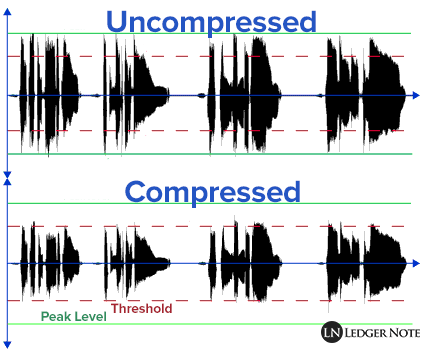
\includegraphics[scale=0.42]{comp.png}
	\end{figure} 
\end{frame}

\begin{frame}{Compression}
  \begin{itemize}
  \item {
    The figure is a block diagram representation of the operations involved in compressing a single channel.
  }
  \item{
  	Generally, stereo or multiple channels are compressed separately.
  }
  \end{itemize}
  \begin{figure}
		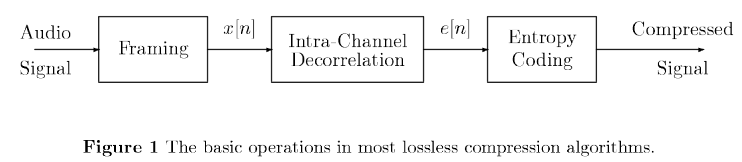
\includegraphics[scale=0.42]{fig1.png}
	\end{figure}  
\end{frame}

\section{ Basic principles of lossless compression}
\subsection{Framing}
\begin{frame}{Basic principles of lossless compression}{Framing}
	\begin{itemize}[<+->]
		\item{
			Framing provides editibility, a very important property for the signal to have in applications dealing with digital audio.
		}
		\item{
			It is important to quickly be able to edit a compressed bit stream.
		}
		\item{
			For practical purposes, the signal is divided into time frames of equal length.
		}
		\item{
			Each frame has a header containing the compression parameters. These can change on a frame-to-frame basis to follow the changing characteristics of the signal.
		}
		\item{
			If the frames are too short, the headers can generate a significant overhead.
		}
		\item{
			If the frames are too long, we lose editibilty.
		}
		\item{
			The most commonly used algorithms use a 13-26 ms time frame durations, translating into 576-1152 samples at 44.1 kHz.
		}
	\end{itemize}
\end{frame}

\subsection{Intra-channel decorrelation}
\begin{frame}{The basic principles of lossless compression}{Intra-channel decorrelation}
	\begin{itemize}[<+->]
		\item{
			The purpose of this step is to remove redundancy by decorrelating the samples within a frame.
		}
		\item{
			2 approaches:
		}
		\begin{enumerate}
			\item{
				Modified linear predictive modelling of the signal.
			}
			\item{
				Obtaining a low bit-rate quantized or lossy representation of the signal, compute the difference between the signals and losslessly compress the computed signal.
			}
		\end{enumerate}
	\end{itemize}
\end{frame}


\begin{frame}{Intra-channel decorrelation}{Linear predictive model}
	\begin{figure}
		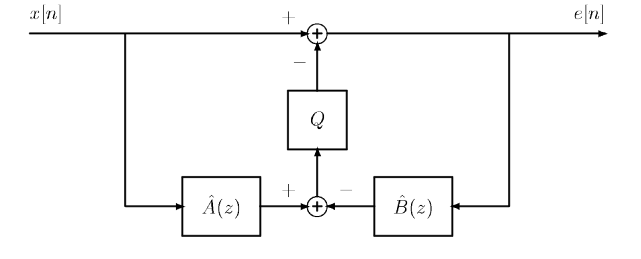
\includegraphics[scale=0.42]{response.png}
	\end{figure}
	\begin{figure}
		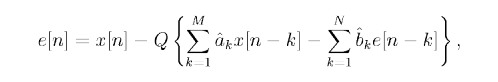
\includegraphics[scale=0.42]{formula.png}
	\end{figure}
\end{frame}

\subsection{Entropy coding}
\begin{frame}{The basic principles of lossless compression}{Entropy coding}
	\begin{itemize}[<+->]
		\item{
			Entropy coding removes redundancy from the residual signal.
		}
		\item{
			No information is lost during the process.
		}
		\item{
			Three widely used methos: Huffman coding, run length coding, Rice conding.
		}
		\item{
			We will discuss the less known of the three, Rice coding.
		}
	\end{itemize}
\end{frame}
\begin{frame}{Entropy coding}{Rice coding}
	\begin{itemize}
		\item{
			Rice coding is characterized by one parameter (m).
		}
		\item{
			In this type of coding, a number is divided into 3 parts: a sign bit, the m low-order bits, and the remaining higher-order bits.
		}
		\item{
			The bit sign is self-explanatory, the second part consists of the m least significant bits of the binary representation of the number's absolute value, and the third part is made of N consecutive zeros, where N has the same binary representation of the yet unused most significant bits; a 1 bit is inserted to terminate the sequence.
		}
		\item{
			The table below show the Rice code representation for parameter m=3.
		}
	\end{itemize}
	\begin{figure}
		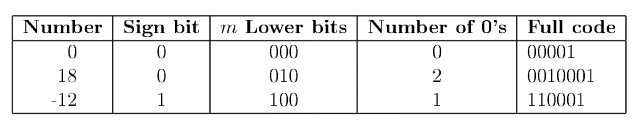
\includegraphics[scale=0.42]{rice_coding.png}
	\end{figure}  
\end{frame}

\section{Performance evaluation}
\begin{frame}{Performance evaluation}{Test suite}
	\begin{itemize}
		\item{
			All of the tracks are in CD format (44.1 kHz, stereo, 16 bits).
		}
	\end{itemize}
	\begin{figure}
		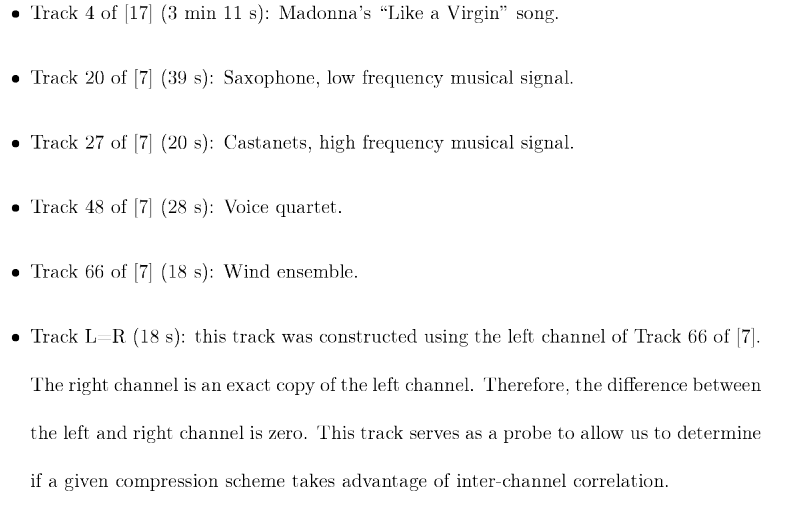
\includegraphics[scale=0.35]{tracks.png}
	\end{figure}  
\end{frame}
\begin{frame}{Performance evaluation}{Results}
	\begin{figure}
		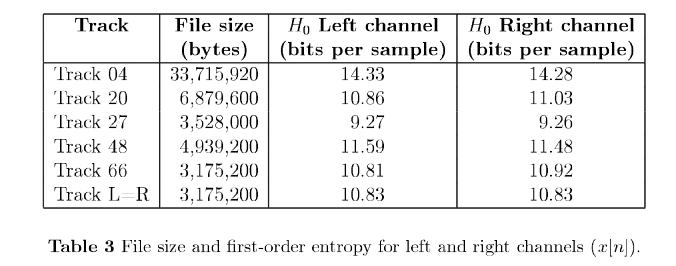
\includegraphics[scale=0.45]{results.png}
	\end{figure} 
\end{frame}
\begin{frame}{Performance evaluation}{Results}
	\begin{figure}
		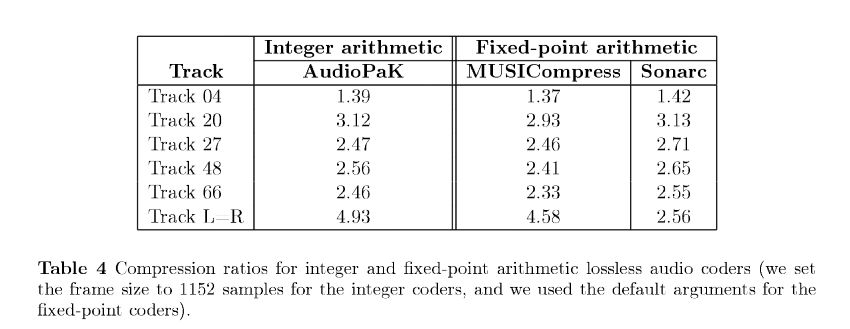
\includegraphics[scale=0.35]{results2.png}
	\end{figure} 
\end{frame}
\begin{frame}{Performance evaluation}{Results}
	\begin{figure}
		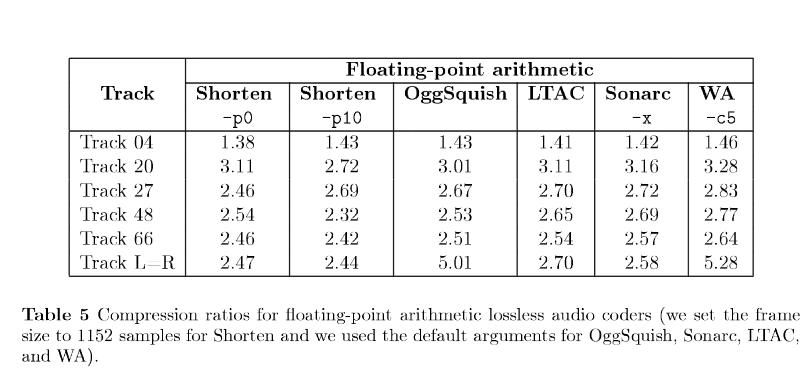
\includegraphics[scale=0.35]{results3.png}
	\end{figure} 
\end{frame}

\begin{frame}{Performance evaluation}{The data}
	\begin{itemize}[<+->]
		\item{
			The data in tables 4 and 5 is very revealing. Firstly, we note that the compression ratios obtained by various state-of-the-art algorithms are quite similar.
		}
		\item{
			The data for Track R=L shows which of the algorithms attempts to take advantage of intra-channel dependencies in a way that works best when the two channels are tightly correlated (in this case they are the same).
		}
		\item{
			Finally, the tests show that WA with the -c5 consistently gives the best compression throughout the 6 tracks.
		}
	\end{itemize}
\end{frame}

% Placing a * after \section means it will not show in the
% outline or table of contents.
\section*{Summary}

\begin{frame}{Summary}
  \begin{itemize}[<+->]
  \item
    This study found that the \alert{currently available compression technology} has \alert{reached a limit} in what we can achieve in \alert{lossless audio compression}.
  \item
    Furthermore, in spite of the \alert{wide range of approaches and complexities} of the differenet compressors, they all \alert{perform similarly} on the same audio signals, generally with less than one bit per sample in difference.
  \item
    It is noteworthy that HP's AudioPaK has similar performance to other modern compressors while keeping the complexity and number of arithmetic operations down. It is likely that upcoming compressor designs will focus on reducing algorithm complexity.
  \end{itemize}
  
\end{frame}

\end{document}


